\section{Motivation}
\label{sec:motivation}

本文工作的背景问题:1. 监控工具可以监控的指标有非常多种,需要熟练的技术知识才能分析这些指标;2. 指标太多不利于直接发现最关键的性能瓶颈,
需要一定的经验知识作为辅导;3. 数学模型的建立有助于评估性能,但是精确的模型的建立及理解都很困难,对模型建立者和使用者都需要
对GPU架构有深刻理解。

\begin{figure}[!t]
\centering
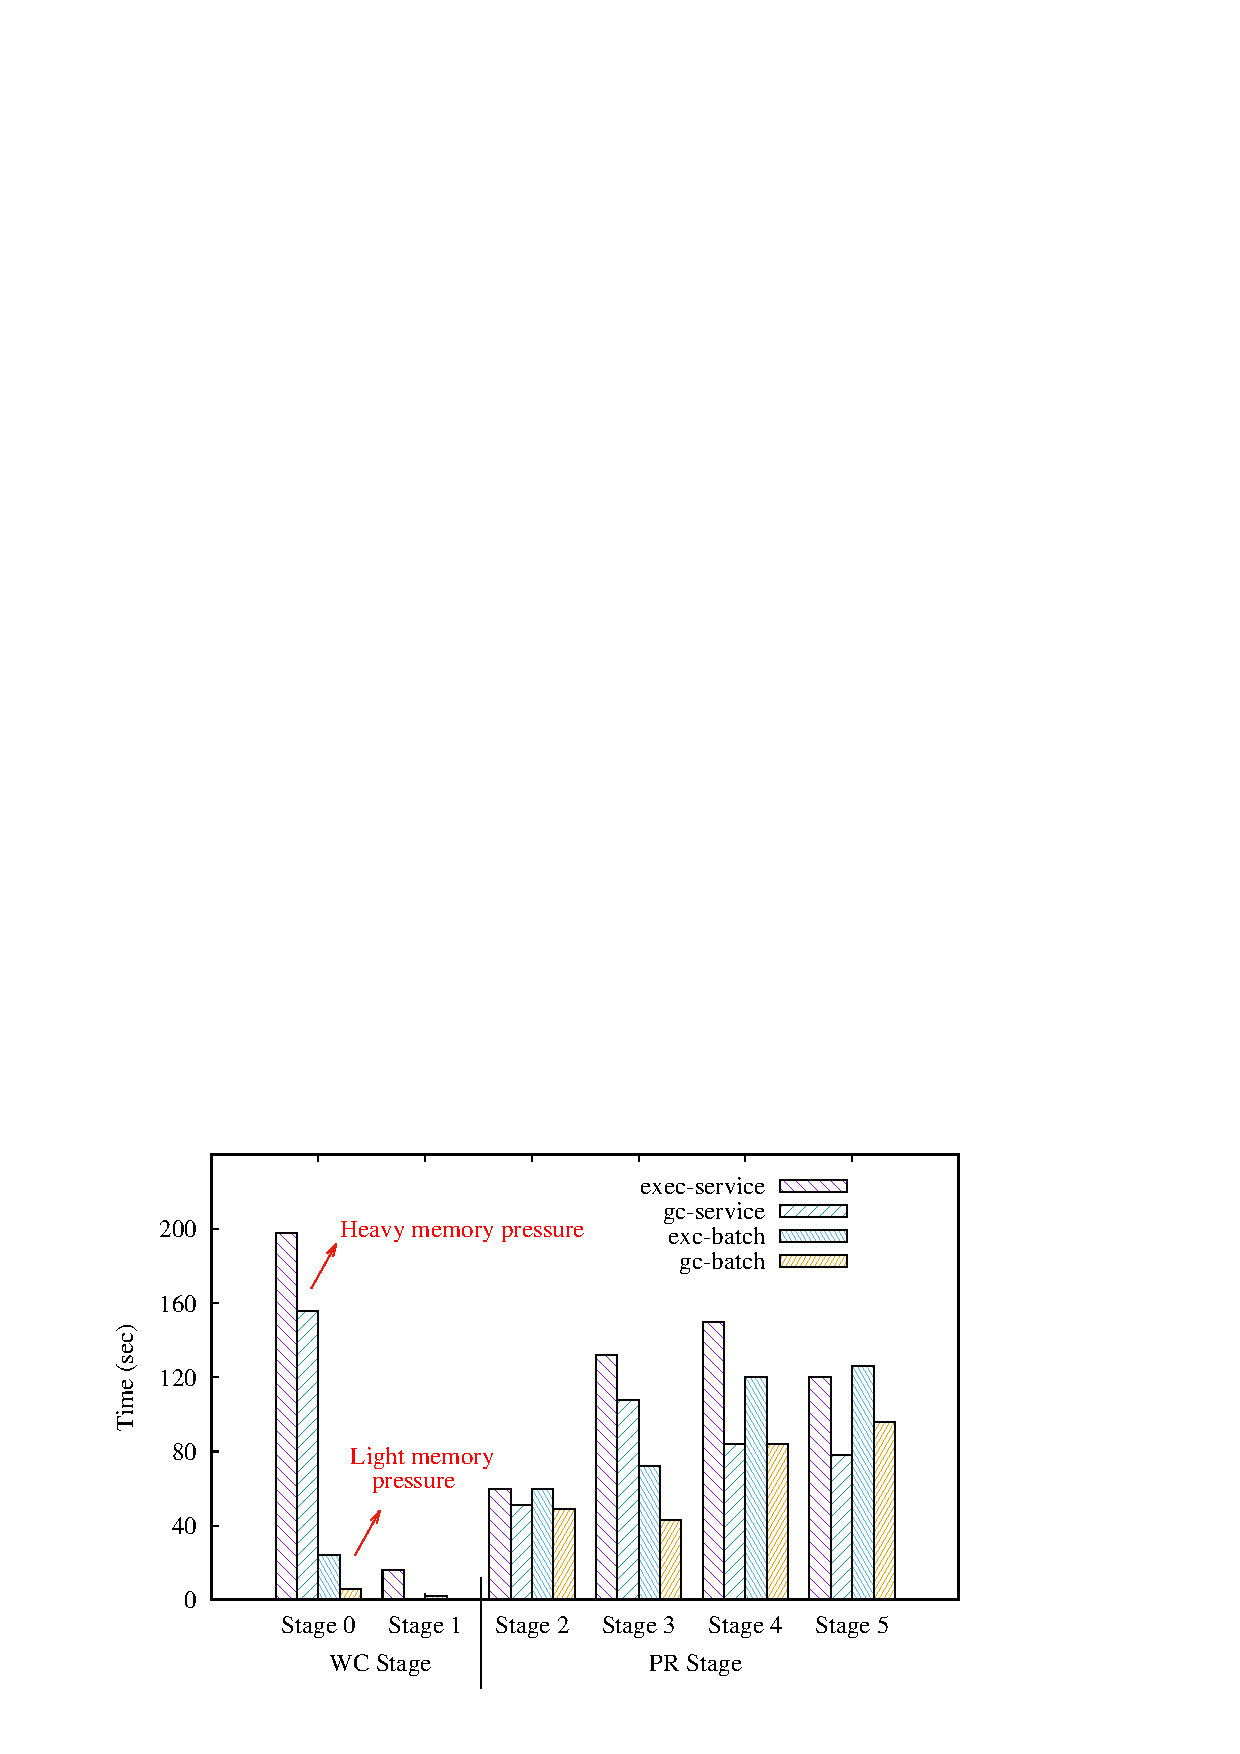
\includegraphics[width=0.4\textwidth]{motivation-exec-gc.pdf}
%\vspace{-2mm}
\caption{WC suffers memory pressure from PR}
%\vspace{-6mm}
\label{fig:memorypressure}
\end{figure}

 
